\section{Methodology}
\label{sectino:Methodology}
This study employs the MaSTr1325 dataset to train a model using Bayesian SegNet, aiming to deliver semantic 
segmentation results for USVs while also quantifying uncertainty. This approach addresses the issue of dataset 
scarcity by enhancing model robustness. Additionally, the model's performance in unfamiliar environments is 
validated using the OASIs dataset. The following sections will detail the dataset preparation, the principles 
underlying Bayesian SegNet, the techniques for uncertainty estimation, and the evaluation metrics.

\subsection{Dataset Preparation}
The study employs two datasets, MaSTr1325 \cite{MaSTr1325} and OASIs \cite{OASIs}. While both datasets provide 
per-pixel annotations, their labelling schemes differ, as detailed in Table \ref{tab:annot-diff}. The annotation 
scheme followed in this research is based on MaSTr1325, which categorizes images into three classes: obstacles 
and environment, water, and sky. Therefore, it is necessary to modify the annotations in the OASIs dataset to 
align with this classification scheme. The "Sea" category in the OASIs dataset is mapped to the "Water" category, 
while the "Land" and "Sea Object" annotations correspond to the "Obstacle and environment" category. However, 
aligning the "Sky" category necessitates some adjustments.

% table
\begin{table}[h!]
    \centering
    \caption{Annotations of MaSTr1325 and OASIs datasets.}
    \label{tab:annot-diff}
    \begin{tabular}{c|c|c|c}
    \textbf{Dataset} & \textbf{Annotation Format} & \textbf{Pixel Value} & \textbf{Pixel Mapping} \\ \hline
    \multirow{4}{*}{MaSTr1325 \cite{MaSTr1325}} & \multirow{4}{*}{Indexed Image (png)} & 0 & Obstacles and environment \\ \cline{3-4}
    & & 1 & Water \\ \cline{3-4}
    & & 2 & Sky \\ \cline{3-4}
    & & 3 & Ignore region \\ \hline
    \multirow{4}{*}{OASIs \cite{OASIs}} & \multirow{4}{*}{Grayscale Image (png)} & 0 & Others \\ \cline{3-4}
    & & 50 & Sea \\ \cline{3-4}
    & & 100 & Land \\ \cline{3-4}
    & & 150 & Sea Object \\ \hline
    \end{tabular}
\end{table}

The OASIs dataset does not include annotations for the "Sky" category, but in most cases, the "Others" category in 
OASIs corresponds to the "Sky" category. However, there are situations where the camera captures the vessel's hull. 
In the OASIs dataset, the hull is classified under the "Others" category, whereas in the MaSTr1325 dataset, even 
a small portion of the USV hull is annotated as "Obstacle and environment". The comparison of annotations related to 
the vessel hull are illustrated in Fig.\ref{fig:vesselhull}. 
\begin{figure}[ht]
    % MaSTr1325
    \centering
    \begin{subfigure}[b]{0.45\textwidth}
        \centering
        \includegraphics[width=\textwidth]{figures/MaSTr1325/vessul-hull.png}
        \caption{}
    \end{subfigure}
    % OASIs
    \centering
    \begin{subfigure}[b]{0.45\textwidth}
        \centering
        \includegraphics[width=\textwidth]{figures/OASIs/vessul-hull.png}
        \caption{}
    \end{subfigure}
    \caption{The Annotation of USV hull on different datasets: (a) MaSTr1325 Dataset with USV hulls, 
    (b) OASIs Dataset with USV and cargo ship hulls.}
    \label{fig:vesselhull}
\end{figure}

Since the annotations cannot be modified, these portions of the data had to be excluded. After excluding 
annotations that include the vessel hull, the "Others" category in the OASIs dataset can be remapped to the "Sky" 
category. Additionally, the images captured from the perspective of cargo ship significantly differ from those taken 
from the USV perspective. Therefore, these two perspectives were separated and used independently for validation. 
After remapping the OASIs dataset annotations to an indexed image format, they can be directly applied for validation.

\subsection{Bayesian SegNet for Semantic Segmentation}
This study utilizes Bayesian SegNet for USV semantic segmentation. Accordingly, this section will explain 
the SegNet Architecture and principles of Dropout Variational Inference, followed by an overview of uncertainty 
estimation. The flow chart of utilizing Bayesian SegNet for semantic segmentation is illustrated in Fig.
\ref{fig:flowchart}
% figure
\begin{figure}[ht]
    \centering
    \includegraphics[width=0.9\textwidth]{figures/flowchart.png}
    \caption{Flow chart on semantic segmentation of Bayesian SegNet.}
    \label{fig:flowchart}
\end{figure}

SegNet consists of an encoder and a decoder network, with a final output layer. The encoder is made up of 13 
convolutional layers, derived from the VGG16 architecture by removing the fully connected layers. The decoder 
network mirrors the encoder, effectively reversing its operations. The final output layer uses the softmax function 
to produce per-pixel point estimates of classes. Due to the removal of fully connected layers, SegNet is 
significantly more efficient than networks like FCN and DeconvNet that include such layers. Additionally, by 
reusing max-pooling indices, SegNet enhances boundary delineation, which is crucial for improving boundary accuracy 
in semantic segmentation tasks \cite{SegNet}.

 Dropout variational inference is utilized in the Bayesian SegNet architecture to provide probabilistic estimates. 
 In the Bayesian paradigm, the posterior distribution is computed based on the prior, likelihood, and evidence in 
 (\ref{eq:bayes-paradigm}). 

\begin{equation}
    P(\mathbf{W}\mid \mathcal{D})=\frac{P(\mathcal{D}\mid \mathbf{W})P(\mathbf{W})}{P(\mathcal{D})}=\frac{P(\mathcal{D},\mathbf{W})}{\int_{\mathbf{W}} P(\mathcal{D},\mathbf{W}^{\prime})d\mathbf{W}^{\prime}}
    \label{eq:bayes-paradigm}
\end{equation}
\vspace{2mm}

$\mathbf{W}$ represents the weights of the network connections, while $\mathcal{D}$ denotes the training dataset, 
which consists of a series of inputs $\mathbf{X}=\{\mathbf{x}_{1},...,\mathbf{x}_{N}\}$ and their corresponding 
labels $\mathbf{Y}=\{\mathbf{y}_{1},...,\mathbf{y}_{N}\}$.

In contrast, VI involves defining a variational distribution $q_{\phi}(\mathbf{W})$ with parameters $\phi$ to 
approximate the posterior distribution. This method seeks to minimize the Kullback-Leibler divergence ($\mathbb{D}_{\text{KL}}$)
\cite{kldivergence} between the variational distribution and the true posterior distribution to achieve a close 
approximation. The optimal value of the parameter $\phi^*$ is given by (\ref{eq:phi-optimal}).\\
\begin{equation}
    \phi^* = \arg \min_{\phi} \mathbb{D}_{\text{KL}}(q_{\phi}(\mathbf{W}) \parallel P(\mathbf{W}\mid \mathcal{D}))
    \label{eq:phi-optimal}
\end{equation}

In BDL, dropout is treated as part of the variational posterior in convolutional layer $i$ with dimension 
$K\text{ x }K$. The weight matrix $\mathbf{W}_i$ is calculated by applying dropout to the variational parameters 
$\mathbf{M}_i$ and vectors of Bernoulli-distributed random variables $z_i$, as shown in (\ref{eq:dropout}). Although 
the dropout probability $p_i$ can be optimized, it is fixed at 0.5 in this study. \\
\vspace{1mm}
\begin{equation}
\begin{aligned}
    &z_{i,j}\sim\mathrm{Bernoulli}(p_i)\mathrm{~for~}j=1,...,K_i,\\
    &\mathbf{W}_i=\mathbf{M}_i\cdot\mathrm{diag}(\mathbf{z}_i),
    \label{eq:dropout}
\end{aligned}
\end{equation}
\vspace{2mm}

For classification tasks, obtaining the per-pixel labelled image and uncertainty requires multiple Monte Carlo 
samples. The segmentation result is derived from the mean of the output layer across $T$ times of Monte Carlo samples, 
as indicated in (\ref{eq:mc-output}). \\
\vspace{1mm}
\begin{equation}
    p(y=c|\mathbf{x},\mathcal{D})\approx\frac{1}{T}\sum_{t=1}^{T}\mathrm{Softmax}(\mathbf{f}^{\widehat{\mathbf{W}}_{t}}(\mathbf{x}))
    \label{eq:mc-output}
\end{equation}
\vspace{2mm}

In this context, $p(y=c|\mathbf{x},\mathcal{D})$ represents the probability of the output $y$ belonging to the 
annotated class $c$ given the input $x$ after training the model. In this study, the annotation classes are defined 
as $c \in C = \{0,1,2,4\}$. Additionally, $\widehat{\mathbf{W}}_{t}$ denotes the convolutional layer weights 
corresponding to the $\text{t}^{\text{th}}$ sample, which have been adjusted according to the dropout variational 
parameters. 

Additionally, Monte Carlo sampling facilitates the calculation of both epistemic and aleatoric uncertainty within 
the model. Epistemic uncertainty refers to the uncertainty in the model parameters and reflects the model's 
understanding of the data distribution. This type of uncertainty, which arise from the marginal posterior distribution 
of the weights, can be mitigated by acquiring more training data. In contrast, aleatoric uncertainty represents the 
inherent noise within the data itself. This type of uncertainty is intrinsic and cannot be reduced by increasing the 
amount of training data. 

It is crucial to estimate both types of uncertainty in semantic segmentation. The estimation formulas for uncertainty 
are illustrated in (\ref{eq:un-est}). Monte Carlo sampling allows for the calculation of the standard deviation 
$\sigma_c$ for each pixel across all classes. By aggregating these deviations, the total standard deviation can be 
obtained to reflect the overall model uncertainty. Aleatoric uncertainty, on the other hand, is assessed by measuring 
the entropy of the distribution. $p_{c}$ represents the probabilistic estimate for class $c$ obtained through Monte 
Carlo sampling. \\
\vspace{-2mm}
\begin{equation}
\begin{aligned}
    \mathbf{EU} = \sum_{c}^{C} \sigma_{c} \ , \quad
    \mathbf{AU} = -\sum_{c}^{C} p_{c} \operatorname{log} p_{c}
    \label{eq:un-est}
\end{aligned}
\end{equation}


\subsection{Evaluation Metrics for Marine Semantic Segmentation}
In semantic segmentation, evaluation metrics plays a crucial role in evaluating model performance. An effective 
metrics facilitates the comparison of different models and enhances the reproducibility of research outcomes. In 
the domain of UGVs, evaluation metrics typically use mean Intersection over Union (mIoU) as the primary evaluation 
metric \cite{CamVid}, \cite{Cityscapes}. However, for marine semantic segmentation, the evaluation protocol must 
address the two distinct challenges faced by USVs: the water edge (shoreline/horizon) detection and the obstacle 
detection \cite{usvbenchmark}. Since the MaSTr1325 dataset lacks shoreline information \cite{MaSTr1325}, this study 
concentrates solely on evaluating the performance of obstacle detection, utilizing metrics of precision 
($\mathbf{Pr}$), recall ($\mathbf{Re}$), and their harmonic mean ($\mathbf{F1}$), as shown in (\ref{eq:metric}).\\
\begin{align}
    \mathbf{Pr} = \frac{TP}{TP+FP} \ , \quad \mathbf{Re} = \frac{TP}{TP+FN} \ , \quad \mathbf{F1} = \frac{2\cdot\mathbf{Pr}\cdot\mathbf{Re}}{\mathbf{Pr}+\mathbf{Re}}
    \label{eq:metric}
\end{align}

True Positive ($TP$) refers to instances where the model correctly identifies a pixel as belonging to the positive 
class. Specifically, for obstacle detection in marine semantic segmentation, a pixel is labeled as a $TP$ when both 
the model's output and the corresponding ground truth annotation are 0. On the other hand, False Positive ($FP$) 
refers to instances where the model incorrectly identifies a pixel as belonging to the positive class. In this 
context, a pixel is labelled as a $FP$ when the model's output is 0, but the corresponding ground truth annotation 
indicates otherwise. Similarly, False Negative ($FN$) refers to instances where the model fails to identify a pixel 
as belonging to the positive class. Here, a pixel is labelled as a $FN$ when the ground truth annotation is 0, but 
the corresponding model's output indicates otherwise.
